\documentclass[11pt]{article}
\pdfinfoomitdate=1
\pdftrailerid{}
\pdfsuppressptexinfo=15
\usepackage[T1]{fontenc}
\usepackage[utf8]{inputenc}
\usepackage{lmodern}
\usepackage[margin=1in]{geometry}
\usepackage{amsmath,amssymb,amsthm,mathtools}
\usepackage{microtype}
\usepackage{enumitem}
\usepackage{xcolor}
\usepackage{tikz}
\usetikzlibrary{positioning,arrows.meta}
\usepackage{hyperref}
\hypersetup{colorlinks=true,linkcolor=blue!45!black,citecolor=blue!45!black,urlcolor=blue!45!black,pdftitle={An isomorphism of the free group factors},pdfauthor={OpenAI}}
\numberwithin{equation}{section}
\newtheorem{theorem}{Theorem}[section]
\newtheorem{lemma}[theorem]{Lemma}
\newtheorem{proposition}[theorem]{Proposition}
\newtheorem{corollary}[theorem]{Corollary}
\theoremstyle{definition}
\newtheorem{definition}[theorem]{Definition}
\theoremstyle{remark}
\newtheorem{remark}[theorem]{Remark}
\newcommand{\F}{\mathbb F}
\newcommand{\R}{\mathbb R}
\newcommand{\C}{\mathbb C}
\newcommand{\N}{\mathbb N}
\newcommand{\ii}{\mathrm i}
\newcommand{\e}{\delta_e}
\DeclareMathOperator{\tr}{tr}
\DeclareMathOperator{\Tr}{Tr}
\DeclareMathOperator{\Cat}{Cat}
\newcommand{\norm}[1]{\left\lVert #1\right\rVert}
\newcommand{\normtwo}[1]{\left\lVert #1\right\rVert_2}
\newcommand{\abs}[1]{\left\lvert #1\right\rvert}
\setlength{\emergencystretch}{2em}
\title{An isomorphism of the free group factors}
\author{OpenAI}
\date{September 23, 2026}
\begin{document}
\maketitle
\begin{abstract}
We solve the free group factor isomorphism problem affirmatively by proving
that $L(\F_2)$ and $L(\F_3)$ are isomorphic as tracial von Neumann algebras.
The classical free group factor alternative then implies that all interpolated
free group factors, including $L(\F_\infty)$, are isomorphic and have
fundamental group $\R_{>0}$.
\end{abstract}

\section{Introduction}
For a discrete group $G$, its group von Neumann algebra is
\[
 L(G)=\{\lambda(g):g\in G\}'',\qquad
 (\lambda(g)\xi)(h)=\xi(g^{-1}h),\quad \xi\in\ell^2(G),
\]
with canonical trace $\tau(x)=\langle x\delta_e,\delta_e\rangle$.
Write $\F_n$ for the free group on $n$ generators and $\F_\infty$ for the free group on countably infinitely many generators. The free group factors arose in Murray and von Neumann's foundational work \cite{murray_vonneumann1943}. Their nonhyperfiniteness distinguished them from the hyperfinite factor, but did not distinguish their ranks; see the historical account in \cite[p.~518]{radulescu1992}. The question whether $L(\F_m)$ and $L(\F_n)$ are isomorphic for distinct $m,n\geq2$ became a central problem in the classification of finite factors. Dykema's introduction \cite[p.~123]{dykema1994} records the early history and credits Kadison with raising the rank-isomorphism question.

Free probability supplied a way to study these factors through their generating distributions. Voiculescu developed the reduced-free-product framework \cite{voiculescu1985} and its semicircular and circular models \cite{voiculescu1990}. His compression results showed that the fundamental group of $L(\F_\infty)$ contains every positive rational, and R\u adulescu extended this to every positive real number \cite{radulescu1992}. Dykema and R\u adulescu independently constructed the interpolated factors $L(\F_r)$ for real $r>1$ and established their amplification calculus \cite{dykema1994,radulescu1994}. These results relate changes of rank to normalized corners. They also give a dichotomy: the interpolated free group factors are either all isomorphic or pairwise nonisomorphic. The version including the infinite parameter is due to R\u adulescu \cite[Corollary~4.7]{radulescu1994}; see also the precise restatement in \cite[Theorem~1.1]{goldbring_pi2025}.

The amplification calculus thus links rank to corner size, while the dichotomy reduces the classification to two alternatives. To choose the isomorphic alternative, it suffices to construct an isomorphism between two distinct finite ranks. Our constructive result is the following rank comparison.
\begin{theorem}[Isomorphism of consecutive ranks]
\label{thm:rank-step}
For every integer $n\geq3$ there is a unital trace-preserving normal
$*$-isomorphism
\[
 L(\F_n)\cong L(\F_{n+1}).
\]
\end{theorem}

The construction gives a freely generating Haar $n$-tuple inside $L(\F_{n+1})$. Applying it at ranks three and four, and then using the established amplification formula, gives the headline conclusion.
\begin{theorem}\label{thm:main}
There exists a unital normal trace-preserving $*$-isomorphism
\[
 \Phi:L(\F_2)\longrightarrow L(\F_3).
\]
\end{theorem}

This gives an affirmative solution to the free group factor isomorphism problem. Together with the classical dichotomy, this proves that all interpolated free group factors, including the infinite-rank factor, are isomorphic. Their fundamental groups are therefore $\R_{>0}$. We state and prove these consequences in Corollary~\ref{cor:all-interpolated}; the constructive rank comparison itself does not use interpolation.

Free entropy offered another approach to distinguishing ranks. A free semicircular $n$-tuple generates $L(\F_n)$ \cite[Remarks~1.10--1.11]{voiculescu1990} and has free entropy dimension $\delta=n$ \cite[Section~2.4(c),(d)]{voiculescu2002entropy}. Voiculescu asked whether $\delta$ of a finite self-adjoint tuple depends only on the tracial von Neumann algebra it generates \cite[Section~2.6]{voiculescu2002entropy}. Such invariance would distinguish the finite ranks. Our isomorphisms give the opposite conclusion: Corollary~\ref{cor:entropy-dimensions} gives a negative answer and proves the same failure for $\delta_0,\delta^*$, and $\delta^\star$. Each of the four dimensions attains every integer value $n\geq2$ on finite self-adjoint generating tuples of $L(\F_2)$. The proof transports semicircular tuples for the microstates dimensions $\delta,\delta_0$ and group-algebra tuples for the nonmicrostates dimensions $\delta^*,\delta^\star$; the two tuple families need not coincide.

Fix $n\geq3$. We begin with a freely generating Haar tuple $(A_1,\ldots,A_n,C)$ in $L(\F_{n+1})$ and set $S=\arg(C)$ using bounded Borel functional calculus. For $g\in\F_n$, let $A_g$ denote the corresponding word in $A_1,\ldots,A_n$. Conjugates $A_gSA_g^*$ drive a polynomial differential equation in $C^*(A_1,\ldots,A_n,S)$. A formal trace identity and analyticity of the actual solutions' moments prove moment preservation. The resulting maps descend through the relations among the generators, preserve the operator norm, and extend to normal trace-preserving automorphisms.

The coefficients are finitely supported real vectors $h_j\in\ell^2(\F_n)$, extended to group words by the cocycle rule
\[
 D_{x_j}=h_j,\qquad D_{gb}=D_g+\lambda(g)D_b,
 \qquad \F_n=\langle x_1,\ldots,x_n\rangle.
\]
After trace preservation has been established, a free-sum estimate gives two bounds for the time-one automorphism $\beta_1$ in Proposition~\ref{prop:flow}, with $w\in\F_n$:
\[
 \norm{\beta_1(A_j)-A_j}\leq3\pi\|h_j\|_{\ell^2},\qquad
 \norm{\beta_1(A_w)-CA_w}\leq3\pi\|D_w-\delta_e\|_{\ell^2}.
\]
Thus small generator coefficients keep the tuple nearly fixed, while a cocycle value near $\delta_e$ makes a selected word approximate $CA_w$.

The coefficient problem is solved in Lemma~\ref{lem:small-cocycle}. For each $m\geq1$, we choose a word $w_m$ with $m$ selected nonidentity prefixes $p_1,\ldots,p_m$ forming a free family. With $h_j=0$ for $j\geq2$, its cocycle value is $D_{w_m}=T_mh_1$, where $T_m=1+\sum_{j=1}^m\lambda(p_j)$. An explicit Catalan moment count shows that the spectral measures of $T_mT_m^*/m$ converge to a measure with no atom at zero. A truncated inverse of $T_mT_m^*$ then gives a small $\ell^2$ vector whose image under $T_m$ is close to $\delta_e$. A real-symmetry argument and a final truncation give finitely supported real coefficients, as required by the polynomial flow.

A free-group basis change now yields an automorphism moving each $A_j$ arbitrarily little in operator norm while making a word in the moved $A_j$'s approximate the \emph{old} variable $C$; this is Proposition~\ref{prop:perturbation}. We iterate this step, choosing each future error budget only after the current approximating word has been fixed. The first $n$ coordinates converge in norm, so their joint Haar distribution persists. The complementary coordinate may vary at every stage. Generation is proved separately: the word algebra of the limiting tuple is dense in the ambient tracial $L^2$ space, and the trace-preserving conditional expectation then identifies its von Neumann closure with the entire factor.

The analytic and algebraic ingredients have established predecessors. Voiculescu's cyclomorphy theorem exponentiates trace-preserving polynomial vector fields on algebraically free self-adjoint generators \cite[Theorem~3.8]{voiculescu2002cyclomorphy}. Our flow uses Haar unitaries and a fixed bounded logarithm, so the descent through their relations is proved directly from moments. Guionnet and Shlyakhtenko's free monotone transport constructs isomorphisms by analytic changes of variables for suitable perturbations of semicircular systems \cite{guionnet_shlyakhtenko2014}; the present argument uses small automorphisms and an iteration that changes the size of a generating tuple. The cocycle product rule is the coefficient form of Fox's free differential calculus \cite[\S1, equation~$(1.2)'$]{fox1953}. The support-independent norm estimate for free sums uses the creation, annihilation, and diagonal decomposition underlying reduced-free-product Khintchine inequalities \cite[\S2]{ricard_xu2006}. We give the estimates and moment arguments needed here in full.

A recent preprint of Shlyakhtenko announces identifications of specified Fuchsian group factors with interpolated free group factors \cite{shlyakhtenko2026fuchsian}. Its main construction finds a free complement to a commutator inside $L(\F_2)$, using finite automorphisms and a limiting generation argument. In both constructions the limiting distribution and the generation of the ambient algebra require separate attention. Here the small-cocycle estimate enables absorption of an additional free generator, and the adaptive error budgets preserve the approximations needed for generation. No result from that preprint is used below.

Section~\ref{sec:prelim} supplies the free-probability and representation facts used in the construction. Sections~\ref{sec:flow} and~\ref{sec:cocycle} construct the automorphisms and their coefficients, and Section~\ref{sec:generation} carries out the limiting argument. Section~\ref{sec:amplification} proves Theorem~\ref{thm:main} and its classical consequences. Section~\ref{sec:entropy-dimensions} proves the generator dependence of free entropy dimensions.

\section{Tracial preliminaries and a free-sum estimate}\label{sec:prelim}
Throughout, $(M,\tau)$ is a von Neumann algebra with faithful normal tracial state. We write
\[
 \normtwo{x}=\tau(x^*x)^{1/2},\qquad \norm{x}=\text{operator norm of }x.
\]
The Hilbert space completion of $M$ in $\normtwo{\cdot}$ is $L^2(M,\tau)$, with inner product $\langle x,y\rangle=\tau(y^*x)$, linear in the first variable. Left multiplication gives its faithful normal representation of $M$. A $*$-isomorphism is a bijective complex-linear map preserving multiplication and adjoints. A linear map between von Neumann algebras is \emph{normal} if it is ultraweakly continuous. We use standard finite von Neumann algebra facts, including bounded Borel functional calculus, Kaplansky density, and the trace-preserving conditional expectation onto a von Neumann subalgebra. The expectation extends to the orthogonal projection of $L^2(M,\tau)$ onto the subalgebra's $L^2$ space. Section~\ref{sec:amplification} recalls the amplification convention separately.

A family $(B_i)_{i\in I}$ of unital subalgebras is \emph{free} if, for every integer $r\geq1$ and every choice of elements satisfying the conditions below,
\[
 \tau(b_1\cdots b_r)=0
 \quad\text{whenever}\quad
 b_j\in B_{i_j},\quad \tau(b_j)=0,\quad
 i_j\ne i_{j+1}\ (1\leq j<r).
\]
Freeness of unital $*$-algebras passes to their generated von Neumann algebras. Indeed, bounded strong approximation gives bounded $L^2$ approximation in a finite tracial algebra; telescoping a product shows continuity of its trace under such approximations. Centering the approximants proves the assertion. Freeness also persists when disjoint collections of the free components are grouped: their algebraic spans consist of scalars and reduced products of centered elements, and the same definition applies to the resulting reduced products.

\subsection{Haar tuples and normal isomorphisms}
\begin{definition}
A \emph{freely generating Haar $d$-tuple} in $M$ is a tuple of unitaries $U=(U_1,\ldots,U_d)$ such that $W^*(U)=M$ and
\[
 \tau(U_g)=0\qquad(g\in\F_d\setminus\{e\}).
\]
Here $U_g$ is the evaluation of the reduced group word $g$ in $U$, with inverse letters evaluated as adjoints.
\end{definition}

\begin{lemma}[Identification by a generating Haar tuple]\label{lem:haar-identification}
For a freely generating Haar $d$-tuple $U$ in $M$, the assignment $\lambda(x_j)\mapsto U_j$ extends to a unital normal trace-preserving $*$-isomorphism $L(\F_d)\to M$.
\end{lemma}
\begin{proof}
The vectors $U_g$, indexed by $g\in\F_d$, are orthonormal because
$\tau(U_h^*U_g)=\tau(U_{h^{-1}g})=\mathbf 1_{g=h}$.
They span $L^2(M,\tau)$. To see this, let $\eta$ be orthogonal to their span. Choose $\eta_m\in M$ converging to $\eta$ in $L^2$. The normal functionals $f_m(x)=\tau(\eta_m^*x)$ converge in norm to $f(x)=\langle x,\eta\rangle$, since $\norm{f_m-f}_{M^*}\leq\normtwo{\eta_m-\eta}$. The space $M_*$ of normal linear functionals is norm closed in $M^*$, so $f$ is normal. It vanishes on the ultraweakly dense word algebra and therefore on all of $M$. Thus $\eta=0$.

Consequently the map $V:\ell^2(\F_d)\to L^2(M,\tau)$ with $V\delta_g=U_g$ is unitary. It intertwines $\lambda(x_j)$ with left multiplication by $U_j$. Conjugation by $V$ identifies their double commutants. The double commutant on the right is the faithful normal left representation of $W^*(U)=M$, so this spatial identification gives the claimed isomorphism. It preserves the trace because $V\delta_e=1$.
\end{proof}

In particular, two freely generating Haar tuples of the same size in $M$ are related by a normal trace-preserving automorphism. The component algebras of a Haar tuple are free: expanding centered Laurent polynomials reduces the assertion to the nonidentity group-word trace, and bounded approximation gives freeness of the von Neumann closures.

For completeness, $L(\F_d)$ is a $\mathrm{II}_1$ factor for $d\geq2$. Its canonical trace is $\tau(x)=\langle x\delta_e,\delta_e\rangle$, which is faithful and normal. Every nonidentity reduced word has infinitely many distinct conjugates: choose a letter $a$ whose powers cause no cancellation at either end of $a^kga^{-k}$. At most two of the $2d$ letters are excluded, and the reduced lengths then tend to infinity. Fourier coefficients of a central element are constant on conjugacy classes and form an $\ell^2$ vector, so every coefficient off the identity vanishes. Faithfulness of the tracial representation implies that the center consists of scalars. The infinitely many orthonormal group unitaries show that the factor is infinite-dimensional.

\subsection{Conjugates of a bounded logarithm}
Fix a freely generating Haar tuple $(A_1,\ldots,A_n,C)$, let $\Gamma=\F_n$, and write $A_g$ for the word in the first $n$ variables indexed by $g\in\Gamma$. Put
\begin{equation}\label{eq:logarithm}
 S=\arg(C),\qquad S_g=A_gSA_g^*\quad(g\in\Gamma),
\end{equation}
where the argument takes values in $(-\pi,\pi]$. The bounded Borel functional calculus for normal operators defines this logarithm in $W^*(C)$; see \cite[Theorem~7.1]{haase2020}. Since the spectral distribution of $C$ is uniform on the circle,
\[
 S=S^*,\quad \norm{S}\leq\pi,\quad \tau(S)=0,\quad e^{\ii S}=C,
 \qquad W^*(S)=W^*(C).
\]

\begin{lemma}[Freeness of the conjugate components]\label{lem:conjugates}
The algebras $A_gW^*(C)A_g^*$, $g\in\Gamma$, form a free family. In particular, each $S_g$ is free from the von Neumann algebra generated by all $S_b$ with $b\ne g$.
\end{lemma}
\begin{proof}
Consider a product of centered elements $A_{g_j}c_jA_{g_j}^*$, with $c_j\in W^*(C)$ and $g_j\ne g_{j+1}$. Cyclicity of the trace rewrites its trace as
\[
 \tau\bigl(c_1 A_{g_1^{-1}g_2}c_2\cdots
          A_{g_{r-1}^{-1}g_r}c_r A_{g_r^{-1}g_1}\bigr).
\]
All interior group elements are nonidentity and hence centered. If the last group element is the identity, omit it; otherwise it too is centered. Freeness of $W^*(A_1,\ldots,A_n)$ and $W^*(C)$ makes the displayed trace zero. For a single factor this is simply $\tau(c_1)=0$. The assertion about the other components follows by grouping free subalgebras.
\end{proof}

For a monomial in $A_j,A_j^*$ and $S$, define its \emph{label} as the product in $\Gamma$ of its group symbols, read in order with each occurrence of $S$ ignored.
\begin{lemma}[Group labels and traces]\label{lem:labels}
A monomial with nonidentity label has trace zero. A monomial with identity label can be expressed as a product of variables $S_g$ (or as the constant $1$).
\end{lemma}
\begin{proof}
For the first assertion, combine consecutive group symbols and consecutive powers of $S$. Remove identity group factors. Split each polynomial in $S$ into its scalar trace and a centered part. A term with all alternating factors centered has trace zero by freeness of the group algebra and $W^*(S)$. Removing a scalar factor permits a reduction to fewer alternating factors, without changing the total group label. Induction on the number of factors ends with either a centered alternating product or a single group element whose label remains nonidentity. Both have trace zero.

For the second assertion, successively use $A_g S=S_g A_g$ to move every group factor to the right. The final group factor is exactly the label, and is therefore $1$.
\end{proof}

\subsection{A bound independent of support size}
For a finitely supported real function $k$ on $\Gamma$, set
\[
 s(k)=\sum_{g\in\Gamma}k(g)S_g.
\]
The coefficient norm $\norm{k}_{\ell^2}$ below is distinguished from the tracial $L^2$ norm $\normtwo{\cdot}$ of operators.
The next estimate uses the creation, annihilation, and diagonal decomposition
underlying free-product Khintchine inequalities; see Ricard and
Xu~\cite[Section~2, Lemmas~2.1--2.3 and Corollary~2.4]{ricard_xu2006}.
We include the scalar self-adjoint argument to give an explicit constant
independent of the number of summands.
\begin{lemma}[Norm of a free sum]\label{lem:free-sum}
For every such $k$,
\begin{equation}\label{eq:free-sum}
 \norm{s(k)}\leq K\norm{k}_{\ell^2},\qquad K=3\pi.
\end{equation}
\end{lemma}
\begin{proof}
We prove the more general bound
\begin{equation}\label{eq:general-free-sum}
 \norm{\sum_j z_j}
 \leq 2\Bigl(\sum_j\normtwo{z_j}^2\Bigr)^{1/2}
       +\max_j\norm{z_j}
\end{equation}
for a finite free family of subalgebras and centered self-adjoint $z_j$ in the respective components.

Work in the tracial $L^2$ space of their generated algebra. Freeness identifies this space with the orthogonal sum of the scalar vector and the reduced centered tensor spaces, whose successive component indices are different. To check the identification, take inner products of reduced centered words. If the two letters at the joining point belong to different components, freeness gives zero. If they belong to the same component, split their product into its trace and its centered part; the latter again has zero contribution, while the scalar term shortens both words. Iteration gives orthogonality for different index sequences and the tensor-product inner product for matching sequences. The reduced word span is dense by the argument used in Lemma~\ref{lem:haar-identification}.

Let $P_j$ project onto the reduced tensors beginning with component $j$, and let $L_{z_j}$ denote left multiplication. On $(1-P_j)L^2$, multiplication prefixes $z_j$, so
\[
 B_j=P_jL_{z_j}(1-P_j),\qquad \norm{B_j}\leq\normtwo{z_j}.
\]
The ranges of the $B_j$ are orthogonal. For every vector $\xi$ this gives
\[
 \norm{\sum_jB_j\xi}^2
   =\sum_j\norm{B_j\xi}^2
   \leq\Bigl(\sum_j\normtwo{z_j}^2\Bigr)\norm{\xi}^2.
\]
The blocks in the opposite direction are $B_j^*$, because $z_j$ is self-adjoint. The block $(1-P_j)L_{z_j}(1-P_j)$ is zero. The remaining diagonal blocks $P_jL_{z_j}P_j$ act on mutually orthogonal subspaces; their sum has norm at most $\max_j\norm{z_j}$. Summing these three parts proves \eqref{eq:general-free-sum}, since the left representation is faithful.

Apply this bound to $z_g=k(g)S_g$. Both $\normtwo{S_g}$ and $\norm{S_g}$ are at most $\pi$, and $\max_g\abs{k(g)}\leq\norm{k}_{\ell^2}$. This proves \eqref{eq:free-sum}.
\end{proof}

\section{Trace-preserving polynomial flows}
\label{sec:flow}

Voiculescu's exponentiation theorem turns trace-preserving polynomial
vector fields on algebraically free self-adjoint generators into
one-parameter automorphism groups~\cite[Theorem~3.8]{voiculescu2002cyclomorphy}.
We prove the version needed here directly for Haar unitaries and a fixed
bounded logarithm. The proof treats the unitary relations explicitly
and derives preservation of all evaluated relations from moment invariance.

Retain the notation of Section~\ref{sec:prelim}. Thus
$(A_1,\ldots,A_n,C)$ is a freely generating Haar tuple in the finite
tracial von Neumann algebra $(M,\tau)$,
$\Gamma=\F_n=\langle x_1,\ldots,x_n\rangle$, and
\[
 S=\arg(C),\qquad S_g=A_gSA_g^*,\qquad
 s(k)=\sum_{g\in\Gamma}k(g)S_g.
\]
Write $\R^{(\Gamma)}$ for the finitely supported real functions on
$\Gamma$, and let $\e\in\ell^2(\Gamma)$ be the unit vector at the
identity. All coefficient vectors used in this section are finitely supported.
The left regular action on them is
$(\lambda(g)k)(b)=k(g^{-1}b)$.

Choose real coefficient vectors $h_1,\ldots,h_n$. There is a unique
cocycle $D:\Gamma\to\R^{(\Gamma)}$ satisfying
\begin{equation}
 D_{x_j}=h_j,\qquad D_{gb}=D_g+\lambda(g)D_b.
 \label{eq:flow-cocycle}
\end{equation}
Indeed, set $D_{x_j^{-1}}=-\lambda(x_j^{-1})h_j$ and define the value
on a word by summing the shifted values of its letters. The two terms
associated with an adjacent inverse pair cancel, so the definition
respects reduction. The cocycle identity and uniqueness follow.

The next proposition turns small $\ell^2$ norms of the $h_j$ into
small operator-norm displacements of the generators. For a word
$w\in\Gamma$, a small $\|D_w-\e\|_{\ell^2}$ also makes the
time-one image of $A_w$ close to $CA_w$.

\begin{proposition}[Polynomial flow and displacement bounds]
\label{prop:flow}
There is a one-parameter group $(\beta_t)_{t\in\R}$ of unital
trace-preserving normal $*$-automorphisms of $M$ that fixes $S$ and
whose restriction to
\[
 B=C^*(A_1,\ldots,A_n,S)
\]
is point-norm continuous. Writing $A_j(t)=\beta_t(A_j)$ and evaluating
group words at this tuple, the paths satisfy
\begin{equation}
 \frac{d}{dt}A_j(t)=\ii s_t(h_j)A_j(t),\qquad
 s_t(k)=\sum_{g\in\Gamma}k(g)A_g(t)SA_g(t)^*,\qquad A_j(0)=A_j.
 \label{eq:flow-ode}
\end{equation}
The derivatives here are in operator norm. With $K=3\pi$ as in
\eqref{eq:free-sum}, for every $t\in\R$,
\begin{align}
 \norm{\beta_t(A_j)-A_j}
 &\leq |t|K\|h_j\|_{\ell^2},
 \label{eq:generator-displacement}\\
 \norm{\beta_t(A_w)-\exp(\ii tS)A_w}
 &\leq |t|K\|D_w-\e\|_{\ell^2}
 \qquad(w\in\Gamma).
 \label{eq:word-displacement}
\end{align}
In particular, at $t=1$ the target in
\eqref{eq:word-displacement} is $CA_w$.
\end{proposition}

We first establish a trace identity on a formal polynomial algebra.
This will prove invariance along the actual flow without assuming
freeness of the evolving tuple.

\subsection{The formal derivation and its trace identity}

Let $\mathcal P$ be the complex unital $*$-algebra generated by
unitaries $a_1,\ldots,a_n$ and a self-adjoint symbol $z$, subject only
to these unitary and self-adjoint relations. Put
\[
 z_g=a_gza_g^*,\qquad \sigma(k)=\sum_gk(g)z_g.
\]
Here $a_g$ is the group word in the formal unitaries. Evaluation at
$(A_1,\ldots,A_n,S)$ defines a $*$-homomorphism
$\operatorname{ev}_0:\mathcal P\to B$; we make no assumption about
its kernel.

Define a complex-linear derivation by the rules
\begin{equation}
 \delta z=0,\qquad
 \delta a_j=\ii\sigma(h_j)a_j,\qquad
 \delta a_j^*=-\ii a_j^*\sigma(h_j).
 \label{eq:formal-derivation}
\end{equation}
These rules define a $*$-derivation on $\mathcal P$. The reality of
$h_j$ makes $\sigma(h_j)$ self-adjoint, so the rules respect
adjoints. They also respect the defining unitary relations: for
example,
\[
 \delta(a_j^*a_j)
 =-\ii a_j^*\sigma(h_j)a_j+\ii a_j^*\sigma(h_j)a_j=0,
\]
and the calculation for $a_ja_j^*$ is the same.
The identity
$a_g\sigma(k)a_g^*=\sigma(\lambda(g)k)$ and the cocycle rule give
\begin{equation}
 \delta a_g=\ii\sigma(D_g)a_g,
 \qquad
 \delta z_g=\ii[\sigma(D_g),z_g].
 \label{eq:formal-word-derivative}
\end{equation}
For instance, multiplying the formulas for $g$ and $b$ gives the
formula for $gb$ with coefficient $D_g+\lambda(g)D_b$; inverse
letters are covered by the unitary relations.

\begin{lemma}[Universal initial trace identity]
\label{lem:flow-trace-identity}
For every $p\in\mathcal P$ and every integer $r\geq1$,
\begin{equation}
 \tau\bigl(\operatorname{ev}_0(\delta^r p)\bigr)=0.
 \label{eq:universal-trace-identity}
\end{equation}
\end{lemma}

\begin{proof}
First take $r=1$. Give a monomial its group label by ignoring each
occurrence of $z$ and multiplying the remaining group symbols in
order. Each term of $\sigma(k)$ has label $e$. The replacement
rules~\eqref{eq:formal-derivation} consequently preserve a monomial's
label term by term. If that label is nonidentity,
Lemma~\ref{lem:labels} makes every evaluated derivative term have
trace zero.

An identity-label monomial is a polynomial in the $z_g$. To see
this algebraically, repeatedly use $a_gz=z_ga_g$ to move group
factors to the right; the final group factor is the identity.
Because these are identities in $\mathcal P$ and $\delta$ is a
derivation on that algebra, differentiating this rewriting gives
the same result as differentiating the original monomial.
It is therefore enough to consider
$p=F(z_g:g\in I)$, with $I\subset\Gamma$ finite and $F$ a
noncommutative polynomial.

For a fixed $g\in I$, remove the commuting own-variable term from
the commutator in~\eqref{eq:formal-word-derivative}. Its evaluated
direction is
\[
 \operatorname{ev}_0(\delta z_g)=\ii[Y_g,S_g],\qquad
 Y_g=\sum_{b\ne g}D_g(b)S_b.
\]
The element $Y_g$ is a bounded self-adjoint in
$B_g=W^*(S_b:b\ne g)$, and $W^*(S_g)$ is free from $B_g$ by
Lemma~\ref{lem:conjugates}.

We use the following direct consequence of freeness. If a unital
subalgebra $\mathcal A$ is free from a unital subalgebra
$\mathcal B$ and $U\in\mathcal B$ is unitary, then
$U\mathcal A U^*$ is free from $\mathcal B$. Indeed, conjugating
an alternating product of centered elements from these two
algebras by $U^*$ gives an alternating product of centered
elements from $\mathcal A$ and $\mathcal B$: a fixed centered
$b\in\mathcal B$ becomes $U^*bU$, which is still centered in
$\mathcal B$. Its trace is zero. Conjugation preserves the
marginal law of each element of $\mathcal A$. Since freeness
determines mixed moments from the marginal laws, it follows that
replacing $S_g$ by $US_gU^*$ preserves its joint law with any
fixed collection of elements of $B_g$.

Apply this observation with $U=\exp(\ii uY_g)$ for real $u$.
The scalar function obtained by replacing every occurrence of
$S_g$ in $F$ by $\exp(\ii uY_g)S_g\exp(-\ii uY_g)$ and leaving
all other variables fixed has constant trace. Its derivative at
zero is the trace of the sum over those occurrences with the
direction $\ii[Y_g,S_g]$ inserted. Sum these zero derivatives over
$g\in I$. The product rule and
\eqref{eq:formal-word-derivative} identify the sum exactly with
$\tau(\operatorname{ev}_0(\delta p))$, proving the case $r=1$.
Linearity handles arbitrary finite sums of monomials.

The result just proved is the identity
$\tau\circ\operatorname{ev}_0\circ\delta=0$ on all of
$\mathcal P$. Since $\delta$ maps finite polynomials to finite
polynomials, applying it to $\delta^{r-1}p$ proves
\eqref{eq:universal-trace-identity}. In this application every
derivative of every coefficient polynomial is included. The
auxiliary conjugations above are used only to compute a first
variation at the initial tuple; they need neither lift to motions
of the $a_j$ nor be jointly integrated.
\end{proof}

\subsection{Global solutions and actual moment invariance}

We now solve the polynomial equation globally in $B$ and use
analyticity to turn the initial trace identity into moment invariance.
For a tuple $X=(X_1,\ldots,X_n)$, let $X_g$ denote the reduced
group word evaluated in a $*$-algebra using adjoints for inverse
letters. This notation defines a polynomial even for nonunitary
tuples, so the right side of~\eqref{eq:flow-ode} defines the finite
polynomial vector field
\[
 \mathcal V_j(X)=\ii H_j(X)X_j,
 \qquad
 H_j(X)=\sum_g h_j(g)X_gSX_g^*.
\]

\begin{lemma}[Global solvability in a generated subalgebra]
\label{lem:flow-global-ode}
Let $E$ be any closed unital $C^*$-subalgebra of $M$ containing
$S$, and let $V_1,\ldots,V_n$ be unitaries in $E$. The equation
$X'=\mathcal V(X)$ with $X(0)=V$ has a unique global solution
in $E^n$ that is smooth in norm, and all its coordinates remain unitary.
\end{lemma}

\begin{proof}
Regard $E^n$, with its maximum norm, as a real Banach space.
Adjunction is bounded and real-linear, so $\mathcal V$ is a
finite smooth polynomial map. Its norm and its Lipschitz constant
are bounded on every fixed bounded ball. Picard iteration on a
sufficiently short interval gives a unique local solution;
repeated differentiation makes it smooth.

Each $H_j(X)$ is self-adjoint, even before unitarity is known.
Along a local solution,
\[
 \frac{d}{dt}(X_j^*X_j)
 =-\ii X_j^*H_j(X)X_j+\ii X_j^*H_j(X)X_j=0.
\]
Thus $X_j^*X_j=1$. Such an isometry is unitary in $M$: the
projection $1-X_jX_j^*$ has trace
$1-\tau(X_j^*X_j)=0$, and faithfulness makes it zero.
This equality also holds in $E$, so $\norm{X_j}=1$ throughout
the local solution.

On this unitary trajectory,
\[
 \norm{X_j'}\leq \norm{S}\sum_g|h_j(g)|.
\]
If a maximal interval had a finite endpoint, this bounded
derivative would make the tuple norm-Cauchy as time approached
that endpoint. Its limit lies in the closed algebra $E$ and is
again a unitary tuple. Local existence at the limit continues
the solution, a contradiction. The same argument applies at
either endpoint, giving a global solution. Uniqueness follows
from local uniqueness on overlapping intervals. This
continuation uses completeness and bounded derivative, not
compactness of a bounded ball.
\end{proof}

Apply Lemma~\ref{lem:flow-global-ode} in $E=B$ with initial
tuple $A$. Let $A(t)$ be its solution and let
$\operatorname{ev}_t:\mathcal P\to B$ evaluate the formal
generators at $A(t),S$. Unitarity makes this a well-defined
evaluation on the formal algebra for each $t$.

\begin{lemma}[Moment invariance]
\label{lem:flow-moments}
For every $p\in\mathcal P$ and $t\in\R$,
\begin{equation}
 \tau\bigl(\operatorname{ev}_t(p)\bigr)
 =\tau\bigl(\operatorname{ev}_0(p)\bigr).
 \label{eq:flow-moments}
\end{equation}
\end{lemma}

\begin{proof}
The differential equation and the product rule give, for every
integer $r\geq0$,
\begin{equation}
 \frac{d^r}{dt^r}\operatorname{ev}_t(p)
 =\operatorname{ev}_t(\delta^r p).
 \label{eq:flow-iterated-derivatives}
\end{equation}
We verify that these derivatives give an actual convergent
Taylor expansion for the trace.

Choose fixed polynomial representatives for the derivatives
of the formal letters in~\eqref{eq:formal-derivation}. There
are constants $J\geq1$ and $B_1\geq1$ such that replacing any
one letter by its derivative increases monomial length by at
most $J$ and produces total absolute coefficient sum at most
$B_1$. These constants are finite because the $h_j$ have finite
support. If a representative of $p$ has degree at most $l$, where
$l\geq1$, and total absolute coefficient sum $b_0$, repeated
replacement gives a representative of $\delta^r p$ with degree
at most $l+rJ$ and coefficient sum at most
\[
 b_0 B_1^r\prod_{v=0}^{r-1}(l+vJ).
\]
Let $R=\max(1,\norm{S})$. All the evaluated group letters are
unitary, so~\eqref{eq:flow-iterated-derivatives} implies, uniformly
for real $t$,
\begin{align}
 \frac{1}{r!}
 \left\|\frac{d^r}{dt^r}\operatorname{ev}_t(p)\right\|
 &\leq b_0R^l(B_1R^J)^r
       \frac{\prod_{v=0}^{r-1}(l+vJ)}{r!} \notag\\
 &\leq b_0R^l\bigl[B_1R^J(l+J)\bigr]^r.
 \label{eq:flow-analytic-bound}
\end{align}
The last inequality uses $l+vJ\leq(l+J)(v+1)$.

Set $f_p(t)=\tau(\operatorname{ev}_t(p))$ and
$c_p=B_1R^J(l+J)$. The integral form of Taylor's remainder and
\eqref{eq:flow-analytic-bound} bound the remainder after degree
$r$ at increment $u$ by $b_0R^l(c_p|u|)^{r+1}$. Consequently
$f_p$ is real-analytic near every real time, with positive
radius at least $c_p^{-1}$. By
Lemma~\ref{lem:flow-trace-identity}, all its positive-order
derivatives at zero vanish. It is constant near zero and hence,
by real-analytic continuation on the connected line $\R$,
constant everywhere.

The constants here may depend on the fixed field and on $p$.
No radius common to all polynomials or to different choices of
the $h_j$ is required. The bounds used only unitarity of the
solution and boundedness of $S$; freeness at positive times has
not been assumed.
\end{proof}

\subsection{Surjectivity, normal extension, and estimates}

\begin{proof}[Proof of Proposition~\ref{prop:flow}]
For a fixed real $t$, polynomial evaluation defines a map
\[
 \varphi_t:\operatorname{ev}_0(\mathcal P)
      \longrightarrow B,
 \qquad
 \varphi_t\bigl(\operatorname{ev}_0(p)\bigr)
      =\operatorname{ev}_t(p).
\]
This is well defined. If $\operatorname{ev}_0(p)=0$, then
\eqref{eq:flow-moments} applied to $p^*p$ gives
\[
 \tau\bigl(\operatorname{ev}_t(p)^*
                 \operatorname{ev}_t(p)\bigr)=0,
\]
so faithfulness implies $\operatorname{ev}_t(p)=0$.
Thus any additional relations at the evaluated initial tuple
are respected as a consequence of actual moment invariance.
The map is unital, complex-linear, multiplicative, and
adjoint-preserving because formal evaluation has those
properties.

For an element $b$ of a finite von Neumann algebra with faithful
tracial state,
\[
 \norm{b}
 =\lim_{k\to\infty}\tau((b^*b)^k)^{1/(2k)}.
\]
For completeness, the upper bound is immediate; for the lower
bound, every nonzero spectral projection of $b^*b$ sufficiently
near its norm has positive trace by faithfulness. Applying
\eqref{eq:flow-moments} to $(p^*p)^k$ therefore shows that
$\varphi_t$ is isometric. It extends uniquely to a
trace-preserving isometric $*$-homomorphism on $B$, with range
\[
 B_t=C^*(A_1(t),\ldots,A_n(t),S).
\]
Indeed, its range is closed and is the norm closure of the
polynomials in these time-$t$ generators.

We next prove $B_t=B$, which establishes surjectivity.
Apply Lemma~\ref{lem:flow-global-ode} inside $B_t$ to the
initial tuple $A(t)$, using the same fixed element $S$ and the
same polynomial field. Its global solution, viewed in $M$,
must be $u\mapsto A(t+u)$ by uniqueness. At $u=-t$ it recovers
the original tuple. Thus every $A_j$ belongs to $B_t$, and
$S$ already belongs to $B_t$, giving $B\subseteq B_t$.
The forward construction gives the reverse inclusion. Hence
$\varphi_t$ is a $C^*$-automorphism of $B$ fixing $S$.

Since $\exp(\ii S)=C$, the von Neumann algebra generated by
$B$ is $M$. Its vectors are therefore dense in $L^2(M,\tau)$,
as in the density argument in
Lemma~\ref{lem:haar-identification}. Trace preservation and
surjectivity define a Hilbert-space unitary
\[
 U_t[b]=[\varphi_t(b)]\qquad(b\in B)
\]
on $L^2(M,\tau)$, fixing $[1]$. If $L_b$ denotes left
multiplication, then on the dense set of vectors coming from
$B$,
\[
 U_t L_b U_t^*=L_{\varphi_t(b)}\qquad(b\in B).
\]
The faithful normal left representation identifies the von
Neumann closure of $L(B)$ with $M$. Conjugation by $U_t$
therefore gives a normal $*$-automorphism $\beta_t$ of $M$
extending $\varphi_t$. It is trace-preserving because $U_t$
fixes $[1]$, and it fixes $S$. This normal extension is unique
by ultraweak density of $B$.

The maps form a one-parameter group. For fixed $s$, the path
$t\mapsto\varphi_s(A(t))$ satisfies the same polynomial
equation, because $\varphi_s$ is a bounded $*$-homomorphism
fixing $S$. Its initial tuple is $A(s)$, so uniqueness gives
\[
 \varphi_s(A_j(t))=A_j(s+t).
\]
The equality on the generators and on $S$ yields
$\varphi_s\varphi_t=\varphi_{s+t}$ on $B$, and uniqueness
of normal extension gives $\beta_s\beta_t=\beta_{s+t}$ on
$M$. Also $\beta_0$ is the identity. Norm continuity on
polynomials in the generators follows from the solution
paths; density and the common isometry bound extend it to
point-norm continuity on $B$. No point-norm continuity on
arbitrary elements of $M$ is needed.

It remains to prove the bounds. For each finitely supported
real $k$,
\[
 s_t(k)=\beta_t(s(k)),\qquad
 \norm{s_t(k)}=\norm{s(k)}\leq K\|k\|_{\ell^2}
\]
by~\eqref{eq:free-sum}. Integrating
$\norm{A_j'(t)}\leq K\|h_j\|_{\ell^2}$ between zero and
$t$ proves~\eqref{eq:generator-displacement}.

For a fixed $w\in\Gamma$, evaluation of
\eqref{eq:formal-word-derivative} along the flow gives
\[
 \frac{d}{dt}A_w(t)=\ii s_t(D_w)A_w(t).
\]
Moreover $s_t(\e)=S$. Direct differentiation, with the order
of factors retained, yields
\[
 \frac{d}{dt}\bigl(\exp(-\ii tS)A_w(t)\bigr)
 =\ii\exp(-\ii tS)\bigl(s_t(D_w)-S\bigr)A_w(t).
\]
The exterior factors are unitary, so its norm is at most
$K\|D_w-\e\|_{\ell^2}$. Integrating between zero and $t$
and multiplying on the left by $\exp(\ii tS)$ proves
\eqref{eq:word-displacement}.
\end{proof}

\section{A small cocycle with a prescribed word value}
\label{sec:cocycle}

Let $n\geq 3$ and $\Gamma=\F_n$, with free generators
$x_1,\ldots,x_n$.  We use the left regular action on coefficient
vectors,
\[
  (\lambda(g)h)(b)=h(g^{-1}b),
  \qquad g,b\in\Gamma,
\]
and write $\tau_\Gamma(X)=\langle X\e,\e\rangle$ for the canonical
trace on $L(\Gamma)$.  Given finitely supported real vectors
$h_1,\ldots,h_n$, let $D$ be the cocycle determined by
\[
  D_{x_j}=h_j,
  \qquad D_{gb}=D_g+\lambda(g)D_b.
\]
The construction in this section makes both $h_1$ and
$D_w-\e$ small in $\ell^2(\Gamma)$, with all the other generator
coefficients zero. At time one, Proposition~\ref{prop:flow} converts
these two coefficient bounds into operator-norm bounds for the generator
displacement and the error between the moved word and $CA_w$.
The word $w$ and the support of $h_1$ are allowed to depend on the
required accuracy.
This coefficient rule is the cocycle form of Fox's free differential
calculus~\cite[Section~1, equations~$(1.2)'$, (1.5)--(1.6), and
Section~2, equations~(2.1)--(2.2)]{fox1953}:
successive letters contribute their generator coefficients translated
by the preceding prefix.  We use that rule explicitly below.

\begin{lemma}[Small coefficients with a prescribed word value]
\label{lem:small-cocycle}
Let $n\geq 3$ and $\eta>0$.
There exist a word $w\in\Gamma$ and a finitely supported real
coefficient vector $h$ such that the cocycle determined by
\[
  h_1=h,\qquad h_j=0\quad(2\leq j\leq n)
\]
satisfies
\begin{equation}
\label{eq:small-cocycle}
  \|h\|_{\ell^2}<\eta,
  \qquad
  \|D_w-\e\|_{\ell^2}<\eta.
\end{equation}
\end{lemma}

\subsection{Free prefix words}

For $j\geq 1$, set
\begin{equation}
\label{eq:cocycle-prefixes}
  a=x_1,
  \qquad b_j=x_2^j x_3 x_2^{-j},
  \qquad p_0=e,
  \qquad p_j=(a b_1)\cdots(a b_j).
\end{equation}
For $m\geq 1$ also set
\begin{equation}
\label{eq:cocycle-word-operator}
  w_m=p_m a,
  \qquad T_m=1+\sum_{j=1}^m\lambda(p_j).
\end{equation}

\begin{lemma}[Free prefixes and the cocycle value]
\label{lem:cocycle-prefixes}
For each $m\geq 1$, the elements $p_1,\ldots,p_m$ freely generate a
free subgroup of $\Gamma$.  If $h_1=h$ and $h_j=0$ for $j\geq 2$,
then
\begin{equation}
\label{eq:cocycle-word-value}
  D_{w_m}=T_m h.
\end{equation}
\end{lemma}

\begin{proof}
First consider a nonempty reduced word in $b_1,\ldots,b_m$.
Combining consecutive powers with the same index writes it as
\[
  b_{j_1}^{q_1}\cdots b_{j_l}^{q_l},
  \qquad q_i\in\mathbb Z\setminus\{0\},
  \qquad j_i\ne j_{i+1}.
\]
Its expansion in $x_2,x_3$ is
\[
  x_2^{j_1}x_3^{q_1}
  x_2^{j_2-j_1}x_3^{q_2}\cdots
  x_2^{j_l-j_{l-1}}x_3^{q_l}x_2^{-j_l}.
\]
Every displayed $x_3$ power is nonzero, and each intervening $x_2$
power is nonzero.  This word cannot reduce to the identity.
Thus the $b_j$ are a free basis of the subgroup they generate.
The free product decomposition
\[
  \Gamma=\langle a\rangle *\langle x_2,\ldots,x_n\rangle
\]
then shows that $a,b_1,\ldots,b_m$ freely generate their subgroup:
an alternating product of nonidentity elements from
$\langle a\rangle$ and $\langle b_1,\ldots,b_m\rangle$ is also
reduced in the displayed free product.

In the abstract free group on $a,b_1,\ldots,b_m$, the substitution
fixing $a$ and sending each $b_j$ to $a b_j$ has inverse given by
$b_j\mapsto a^{-1}b_j$, again fixing $a$.
Consequently
\[
  u_j=a b_j,\qquad 1\leq j\leq m,
\]
form a free family.  On the abstract free group with free basis
$u_1,\ldots,u_m$, define two endomorphisms by
\[
  \varphi(u_j)=u_1\cdots u_j,
  \qquad
  \psi(u_1)=u_1,
  \qquad
  \psi(u_j)=u_{j-1}^{-1}u_j\quad (j\geq 2).
\]
For every $j$, cancellation gives
\begin{align*}
  \psi\varphi(u_j)
    &=u_1(u_1^{-1}u_2)\cdots(u_{j-1}^{-1}u_j)=u_j,\\
  \varphi\psi(u_j)
    &=(u_1\cdots u_{j-1})^{-1}(u_1\cdots u_j)=u_j
       \quad (j\geq 2),
\end{align*}
and the second identity also holds for $j=1$.
Thus $\varphi$ and $\psi$ are inverse automorphisms.
Since $p_j=u_1\cdots u_j$, this proves the assertion about the
$p_j$.

For the cocycle assertion, the inverse rule
$D_{x_j^{-1}}=-\lambda(x_j^{-1})D_{x_j}$ shows that $D$ vanishes
on the subgroup generated by $x_2,\ldots,x_n$.
In particular, $D_{b_j}=0$.
The positive occurrences of $a$ in $w_m$ have respective prefixes
$p_0,p_1,\ldots,p_m$, and there are no other occurrences of $a$
or $a^{-1}$.
Applying the cocycle identity successively therefore gives
\[
  D_{w_m}=\sum_{j=0}^m\lambda(p_j)h=T_mh.
\]
\end{proof}

\subsection{The spectral measures of the prefix sums}

Put
\begin{equation}
\label{eq:cocycle-positive-operator}
  Q_m=T_mT_m^*,
  \qquad
  \mu_m(B)=\tau_\Gamma\bigl(1_B(Q_m/m)\bigr)
\end{equation}
for Borel sets $B\subseteq[0,\infty)$.
These are probability measures by the spectral theorem and the
normalization of $\tau_\Gamma$.

We seek a small vector $h$ with $T_mh$ close to $\e$. The spectral
limit below has no atom at zero. It will let us choose a small fixed
cutoff in the normalized spectrum and then make $m$ large enough that
the discarded projection has small trace. On the remaining spectrum,
the inverse of $Q_m$ has norm at most a fixed constant times $m^{-1}$.
The inverse bound controls the coefficient norm, while the discarded
trace controls the approximation error.
The Catalan count below is the moment calculation associated with
circular systems in Voiculescu's free-probability framework;
see~\cite{voiculescu1985} and~\cite[Definition~1.9 and Remark~1.11]{voiculescu1990}.
We give the word count and the normalization of the limiting density
explicitly.

\begin{lemma}[Spectral limit of the prefix sums]
\label{lem:cocycle-spectrum}
The measures $\mu_m$ converge weakly to the probability measure
\begin{equation}
\label{eq:cocycle-limit-density}
  d\nu(x)=\frac{1}{2\pi}\sqrt{\frac{4-x}{x}}
           \,1_{(0,4)}(x)\,dx.
\end{equation}
In particular, $\nu(\{0\})=0$.
\end{lemma}

\begin{proof}
Write $V_j=\lambda(p_j)$ and $V_0=1$.
Lemma~\ref{lem:cocycle-prefixes} implies that a word in
$V_1,\ldots,V_m$ and their inverses has trace one if its word in
these free symbols reduces to the identity, and trace zero
otherwise.
This trace rule applies inside the given regular representation.
Indeed, for $H=\langle p_1,\ldots,p_m\rangle$, the spaces
$\ell^2(Ht)$, as $Ht$ ranges over the right cosets of $H$, are
reducing copies of the left regular representation of $H$.
The vector $\e$ lies in the copy $\ell^2(H)$.
Its vector state therefore agrees with the canonical trace of
$H$ on polynomials and on the spectral projections under
consideration.

Fix an integer $r\geq 1$.  Expanding $Q_m^r$ gives
\begin{equation}
\label{eq:cocycle-moment-expansion}
  \tau_\Gamma(Q_m^r)
  =\sum_{i_1,\ldots,i_{2r}\in\{0,\ldots,m\}}
    \tau_\Gamma\bigl(
      V_{i_1}V_{i_2}^*\cdots V_{i_{2r-1}}V_{i_{2r}}^*
    \bigr).
\end{equation}
Each summand is zero or one.  In a summand equal to one, every
nonzero index used must occur at least twice, since a generator
occurring only once cannot disappear under free reduction.
There are therefore at most $r$ distinct nonzero indices.

If exactly $r$ distinct nonzero indices occur, all $2r$ positions
are nonidentity and each index occurs exactly twice.
The two occurrences have opposite exponents, as follows already
by abelianizing the identity word.
Pair the two positions with the same index.  This matching is
unique for the chosen word.
A sequence of adjacent inverse cancellations produces a
noncrossing matching: a pair deleted after other pairs can only
enclose pairs already deleted, and two deleted pairs cannot
cross.
Conversely, a noncrossing matching with opposite exponents at
its endpoints reduces to the identity by deleting an innermost
pair and proceeding by induction.
Every noncrossing perfect matching of $\{1,\ldots,2r\}$ has
opposite parity at the two endpoints of each pair.  To see this,
the positions strictly inside that pair must be matched among
themselves, so their number is even.
The signs in~\eqref{eq:cocycle-moment-expansion} alternate;
therefore every noncrossing perfect matching has the required
opposite signs.

The number of noncrossing perfect matchings is
\[
  \Cat_r=\frac{1}{r+1}\binom{2r}{r}.
\]
For completeness, splitting a matching at the partner of its
first position gives the recurrence
$c_0=1$ and $c_r=\sum_{j=0}^{r-1}c_jc_{r-1-j}$.
Its formal generating series satisfies $C(z)=1+zC(z)^2$,
so the solution with constant term one is
$(1-\sqrt{1-4z})/(2z)$; the binomial expansion gives the displayed
coefficient $\Cat_r$.
For each matching, labeling its $r$ pairs with distinct indices
from $\{1,\ldots,m\}$ gives
\[
  (m)_r=m(m-1)\cdots(m-r+1)
\]
choices, with the value zero when $m<r$.
Ordering the pairs by their first endpoints makes this count
unambiguous, and the uniqueness of the equal-index matching
prevents double counting.
Thus the contribution from exactly $r$ distinct indices is
$\Cat_r(m)_r$.

Every remaining contributing term has at most $r-1$ distinct
nonzero indices.  This includes every term with an identity
summand: such a term has at most $2r-1$ nonidentity positions,
while each index it uses occurs at least twice.
For fixed $r$, there are only finitely many patterns specifying
the identity positions and the partition of the other positions
into equal-index classes.  A pattern with $k\leq r-1$ classes
has at most $m^k$ labelings.  Summing over those patterns gives
an $O_r(m^{r-1})$ bound, with its constant depending only on $r$.
We have proved
\begin{equation}
\label{eq:cocycle-catalan-moments}
  \tau_\Gamma(Q_m^r)
    =\Cat_r(m)_r+O_r(m^{r-1}),
  \qquad
  \int x^r\,d\mu_m(x)\longrightarrow\Cat_r.
\end{equation}

We next justify passage from moments to weak convergence.
For $r=1$, direct expansion gives
$\tau_\Gamma(Q_m)=m+1$, so the first moments of $\mu_m$ are
bounded by two.  Markov's inequality gives tightness on
$[0,\infty)$.
For each fixed integer $r\geq 1$, the moment convergence in
\eqref{eq:cocycle-catalan-moments}, applied also at $r+1$, gives
\[
  \sup_m\int x^{r+1}\,d\mu_m(x)<\infty,
  \qquad
  \sup_m\int_{(R,\infty)}x^r\,d\mu_m(x)
    \leq \frac{1}{R}\sup_m\int x^{r+1}\,d\mu_m(x)
    \longrightarrow 0
\]
as $R\to\infty$.
Consequently, if a subsequence converges weakly to a probability
measure $\mu$, its moments pass to the limit.
More explicitly, apply weak convergence to the bounded continuous
functions $\min\{x^r,R^r\}$ and use the displayed tail bound;
the corresponding bound for $\mu$ follows by first applying
weak convergence to bounded truncations of $x^{r+1}$.
Letting $R\to\infty$ proves
\begin{equation}
\label{eq:cocycle-subsequence-moments}
  \int x^r\,d\mu(x)=\Cat_r\qquad(r\geq 0).
\end{equation}

The density in~\eqref{eq:cocycle-limit-density} realizes these
moments, including the zeroth moment. Write
$B(a,b)=\int_0^1t^{a-1}(1-t)^{b-1}\,dt$ for the Euler beta integral.
The substitution
$x=4t$ and the beta integral give, for every integer $r\geq 0$,
\begin{align*}
  \frac{1}{2\pi}\int_0^4 x^{r-1/2}(4-x)^{1/2}\,dx
    &=\frac{4^{r+1}}{2\pi}
      B\left(r+\frac12,\frac32\right)\\
    &=\frac{(2r)!}{r!(r+1)!}
      =\Cat_r.
\end{align*}
The middle equality follows from
$B(\tfrac12,\tfrac32)=\pi/2$ and the recurrence
$B(a+1,b)=aB(a,b)/(a+b)$.
In particular the density has total mass one.

These moments determine a probability measure on
$[0,\infty)$ uniquely.
Indeed, $\Cat_r\leq 4^r$.  If a measure satisfying
\eqref{eq:cocycle-subsequence-moments} had mass $c>0$ on
$[4+\epsilon,\infty)$ for some $\epsilon>0$, then
\[
  4^r\geq\Cat_r\geq c(4+\epsilon)^r
\]
for every $r$, a contradiction for large $r$.
Its support is therefore contained in $[0,4]$.
On this compact interval, uniform polynomial approximation of
continuous functions shows that equality of all moments implies
equality of the measures.
Every subsequential weak limit is consequently $\nu$.
Tightness now gives weak convergence of the full sequence
$\mu_m$ to $\nu$.
Finally, $\nu$ has the displayed integrable density and thus has
no atom at zero.
\end{proof}

\subsection{Cutoff inversion and finite coefficients}



\begin{proof}[Proof of Lemma~\ref{lem:small-cocycle}]
Use the operators $T_m,Q_m$ and the measures $\mu_m$ above.
Since $\nu(\{0\})=0$, choose a fixed $d>0$ so small that
\[
  \nu([0,d])<\frac{\eta^2}{16}.
\]
The interval $[0,d]$ is closed, so weak convergence and the
Portmanteau inequality give
\[
  \limsup_{m\to\infty}\mu_m([0,d])
     \leq\nu([0,d])<\frac{\eta^2}{16}.
\]
We may therefore choose $m$ sufficiently large that both
\begin{equation}
\label{eq:cocycle-cutoff-choices}
  \mu_m([0,d])<\frac{\eta^2}{8},
  \qquad
  \frac{1}{dm}<\frac{\eta^2}{16}
\end{equation}
hold.  Keep this $d$ and this $m$ fixed for the remainder of the
construction.

Set
\[
  E_m=1_{(dm,\infty)}(Q_m),
  \qquad R_m=f_m(Q_m),
  \qquad
  f_m(x)=
  \begin{cases}
    0,&0\leq x\leq dm,\\
    x^{-1},&x>dm.
  \end{cases}
\]
Thus $R_m$ is a bounded positive operator, with
$\norm{R_m}\leq (dm)^{-1}$.
The spectral theorem gives
\begin{equation}
\label{eq:cocycle-cutoff-identities}
  Q_m R_m=E_m,
  \qquad R_m Q_m R_m=R_m,
  \qquad
  \tau_\Gamma(1-E_m)=\mu_m([0,d]).
\end{equation}
In particular, these operations allow a kernel or arbitrarily
small nonzero spectrum of $Q_m$.
Define the coefficient vector
\[
  h^{(0)}=T_m^*R_m\e\in\ell^2(\Gamma).
\]
Using $Q_m=T_mT_m^*$ in the indicated order gives
\begin{align}
\label{eq:cocycle-cutoff-target}
  T_mh^{(0)}&=E_m\e,\\
\label{eq:cocycle-cutoff-error}
  \|T_mh^{(0)}-\e\|_{\ell^2}^2
    &=\tau_\Gamma(1-E_m)<\frac{\eta^2}{8},\\
\label{eq:cocycle-cutoff-size}
  \|h^{(0)}\|_{\ell^2}^2
    &=\langle R_mQ_mR_m\e,\e\rangle
      =\tau_\Gamma(R_m)
      \leq\frac{1}{dm}<\frac{\eta^2}{16}.
\end{align}

The vector $h^{(0)}$ has real coefficients.
To check this directly, let $J$ denote coefficientwise complex
conjugation on $\ell^2(\Gamma)$.
Each left shift is real in the standard basis, so $J$ commutes
with $T_m,T_m^*$ and $Q_m$, and $J\e=\e$.
Commutation with real polynomials in $Q_m$ extends by uniform
approximation to real continuous functions of $Q_m$.
The continuous functions
\[
  x\longmapsto \min\{1,\max\{0,l(x-dm)\}\},
  \qquad l=1,2,\ldots,
\]
converge pointwise, with a uniform bound, to
$1_{(dm,\infty)}(x)$ on the spectrum of $Q_m$.
Their functional calculi converge strongly to $E_m$, hence
$J$ also commutes with $E_m$.
Finally,
\[
  R_m=E_m g_m(Q_m),
  \qquad g_m(x)=\frac{1}{\max\{dm,x\}},
\]
where $g_m$ is real and continuous on $[0,\infty)$.
Thus $J$ commutes with $R_m$ as well, proving
$Jh^{(0)}=h^{(0)}$.

Real finitely supported coefficient vectors are dense in the
real subspace of $\ell^2(\Gamma)$.
Choose such a vector $h$ with
\[
  \|h-h^{(0)}\|_{\ell^2}
       <\frac{\eta}{4(m+1)}.
\]
The elementary bound $\norm{T_m}\leq m+1$ and
\eqref{eq:cocycle-cutoff-error}--\eqref{eq:cocycle-cutoff-size}
yield
\begin{align*}
  \|h\|_{\ell^2}
    &<\frac{\eta}{4}+\frac{\eta}{4(m+1)}<\eta,\\
  \|T_mh-\e\|_{\ell^2}
    &<\frac{\eta}{\sqrt{8}}+\frac{\eta}{4}<\eta.
\end{align*}
For this finitely supported $h$, form the cocycle with
$h_1=h$ and all other generator values zero, and take $w=w_m$.
Equation~\eqref{eq:cocycle-word-value} gives $D_w=T_mh$, proving
\eqref{eq:small-cocycle}.

The choices have been made in the order $d$, then $m$, then the
finite coefficient approximation.  The last approximation uses
the norm of the already fixed operator $T_m$; the lemma requires
no bound on the support size of $h$ uniform in $\eta$.
\end{proof}

\section{Perturbation and a generating limit}
\label{sec:generation}

We combine the flow estimate with the small-cocycle construction to
approximate the extra generator by a word in a slightly perturbed
$n$-tuple.  We then arrange these approximations so that the limiting
$n$-tuple generates the entire von Neumann algebra.
We call $C$ a \emph{completion} of $A=(A_1,\ldots,A_n)$ when
$(A,C)$ is a freely generating Haar tuple in $M$.

\subsection{One-step perturbation}

\begin{proposition}[Approximating the extra generator in one step]
\label{prop:perturbation}
Let $n\geq 3$, and let $(A_1,\ldots,A_n,C)$ be a freely generating Haar
tuple in a finite von Neumann algebra $(M,\tau)$.  For every
$\varepsilon>0$ there are a trace-preserving normal automorphism
$\alpha$ of $M$ and a word $w\in\F_n$ such that, with
$A_j'=\alpha(A_j)$,
\begin{equation}
\label{eq:perturbation}
 \max_{1\leq j\leq n}\norm{A_j'-A_j}<\varepsilon,
 \qquad
 \norm{A_w'-C}<\varepsilon.
\end{equation}
The tuple $(A_1',\ldots,A_n',C')$, where $C'=\alpha(C)$, is again freely
generating Haar.  Here the target in the second estimate is the
original $C$; the new completion is
\[
 C'=C A_w^*,
\]
where $A_w$ is evaluated on the original $n$-tuple.
\end{proposition}

\begin{proof}
Choose $0<\eta<\varepsilon/K$, with $K=3\pi$ as in
\eqref{eq:free-sum}.  Lemma~\ref{lem:small-cocycle} gives a finitely
supported real coefficient vector $h_1$, with $h_j=0$ for $j\geq2$,
and a word $w\in\F_n$ for which
\[
 \|h_1\|_{\ell^2}<\eta,
 \qquad
 \|D_w-\e\|_{\ell^2}<\eta.
\]
Apply Proposition~\ref{prop:flow} to these coefficients and write
$\beta=\beta_1$.  Its displacement estimates
\eqref{eq:generator-displacement} and \eqref{eq:word-displacement}
give
\[
 \max_j\norm{\beta(A_j)-A_j}<\varepsilon,
 \qquad
 \norm{\beta(A_w)-C A_w}<\varepsilon.
\]
Moreover, $\beta$ fixes $S$ and therefore fixes $C=\exp(\ii S)$.

The free-group basis transformation that fixes the first $n$ symbols
and sends the last symbol $c$ to $c w$ is invertible: its inverse
fixes the first $n$ symbols and sends $c$ to $c w^{-1}$.  By
Lemma~\ref{lem:haar-identification}, it induces a trace-preserving
normal automorphism $\gamma$ of $M$ satisfying
\[
 \gamma(A_j)=A_j \quad(1\leq j\leq n),
 \qquad
 \gamma(C)=C A_w.
\]
Set $\alpha=\gamma^{-1}\circ\beta$.  Since $\gamma$ fixes every
$A_j$ and hence $A_w$, we have the exact identities
\begin{align*}
 \alpha(A_j)-A_j
   &=\gamma^{-1}\bigl(\beta(A_j)-A_j\bigr),\\
 \alpha(A_w)-C
   &=\gamma^{-1}\bigl(\beta(A_w)-C A_w\bigr).
\end{align*}
An automorphism is isometric, so these identities prove
\eqref{eq:perturbation}, with the displayed order of the factors.
The image under $\alpha$ of the original freely generating Haar
tuple is again such a tuple.  Finally,
\[
 C'=\alpha(C)=\gamma^{-1}(C)=C A_w^*,
\]
because $\beta(C)=C$ and
$\gamma(C A_w^*)=C A_w A_w^*=C$.
\end{proof}

\subsection{A generating limit}

We record the elementary continuity estimate that will control the
iteration.  For two $d$-tuples of unitaries $U=(U_1,\ldots,U_d)$ and
$V=(V_1,\ldots,V_d)$, put
\[
 d_2(U,V)=\max_{1\leq j\leq d}\normtwo{U_j-V_j}.
\]
If $v$ is a group word of length $|v|$, telescoping its product gives
\[
 \normtwo{U_v-V_v}\leq |v|\,d_2(U,V).
\]
Indeed, multiplication on either side by a unitary preserves the
tracial $L^2$ norm, and
$\normtwo{U_j^*-V_j^*}=\normtwo{U_j-V_j}$.
Consequently, a finite word polynomial
$F=\sum_{\nu=1}^q c_\nu v_\nu$ satisfies
\begin{equation}
\label{eq:word-polynomial-lipschitz}
 \normtwo{F(U)-F(V)}
 \leq L(F)d_2(U,V),
 \qquad
 L(F)=\sum_{\nu=1}^q |c_\nu|\,|v_\nu|.
\end{equation}
The same telescoping argument also gives continuity in operator norm.

\begin{proof}[Proof of Theorem~\ref{thm:rank-step}]
Fix $n\geq3$ and let $M=L(\F_{n+1})$, with its canonical normalized
trace and canonical freely generating Haar tuple
\[
 (A_1^{(0)},\ldots,A_n^{(0)},C^{(0)}).
\]
Write $A^{(k)}=(A_1^{(k)},\ldots,A_n^{(k)})$.  Choose a sequence
$(y_j)_{j\geq1}$ that is dense in $L^2(M,\tau)$ and consists of
elements of the rational complex group word algebra of the initial
tuple.  Such a sequence exists by
Lemma~\ref{lem:haar-identification}; coefficients in
$\mathbb{Q}+\ii\mathbb{Q}$ make this algebra countable.  Put $r_0=1$.

We construct freely generating Haar tuples $(A^{(k)},C^{(k)})$ and
positive numbers $r_k$ by induction.  Suppose the construction has
reached stage $k-1$, where $k\geq1$.  The choices at stage $k$ are
made in the following order.

First, for each $1\leq j\leq k$, choose a finite linear combination
$F_{j,k}$ of group words in $n+1$ variables such that
\begin{equation}
\label{eq:stage-old-approximation}
 \normtwo{
 F_{j,k}(A^{(k-1)},C^{(k-1)})-y_j
 }<2^{-k}.
\end{equation}
This is possible because the current completed tuple generates $M$
and its group word algebra is dense in $L^2(M,\tau)$.
Let $H_k\geq0$ be a common bound for the finitely many constants
$L(F_{j,k})$ in \eqref{eq:word-polynomial-lipschitz}.  Choose
\begin{equation}
\label{eq:stage-tolerance}
 0<\varepsilon_k<
 \min\left\{\frac{r_{k-1}}2,\,
                  \frac{2^{-k}}{1+H_k}\right\}.
\end{equation}

Next apply Proposition~\ref{prop:perturbation} to
$(A^{(k-1)},C^{(k-1)})$ with tolerance $\varepsilon_k$.
Let $\alpha_k$ and $w_k\in\F_n$ be its automorphism and word, and set
\[
 A_j^{(k)}=\alpha_k(A_j^{(k-1)}),
 \qquad
 C^{(k)}=\alpha_k(C^{(k-1)}).
\]
The new completed tuple is freely generating Haar, and
\begin{equation}
\label{eq:stage-perturbation}
 \max_j\norm{A_j^{(k)}-A_j^{(k-1)}}<\varepsilon_k,
 \qquad
 \norm{A_{w_k}^{(k)}-C^{(k-1)}}<\varepsilon_k.
\end{equation}
In particular, the last expression is close to the old completion,
as needed in \eqref{eq:stage-old-approximation}.

Now define word polynomials in $n$ variables by
\[
 G_{j,k}(X)=F_{j,k}(X,X_{w_k})
 \qquad(1\leq j\leq k).
\]
Since $\normtwo{x}\leq\norm{x}$, equations
\eqref{eq:word-polynomial-lipschitz},
\eqref{eq:stage-old-approximation}, and
\eqref{eq:stage-perturbation} imply
\begin{align}
\label{eq:stage-new-approximation}
 \normtwo{G_{j,k}(A^{(k)})-y_j}
 &\leq
 \normtwo{F_{j,k}(A^{(k)},A_{w_k}^{(k)})
       -F_{j,k}(A^{(k-1)},C^{(k-1)})}
 \notag\\
 &\qquad
 +\normtwo{F_{j,k}(A^{(k-1)},C^{(k-1)})-y_j}
 \notag\\
 &<H_k\varepsilon_k+2^{-k}<2\cdot2^{-k}.
\end{align}
This estimate uses $A_{w_k}^{(k)}$ as a single unitary slot of
$F_{j,k}$.  Thus the tolerance chosen in
\eqref{eq:stage-tolerance} does not depend on the length of the word
that the perturbation subsequently produces.

Finally, let $L_k\geq0$ be a common $L^2$-Lipschitz bound for the
finitely many polynomials $G_{j,k}$, and choose
\begin{equation}
\label{eq:future-budget}
 0<r_k\leq
 \min\left\{\frac{r_{k-1}}2,\,
                  \frac{2^{-k}}{1+L_k}\right\}.
\end{equation}
These constants are finite by
\eqref{eq:word-polynomial-lipschitz}.  They are chosen after $w_k$
is known, so any increase in word length is accommodated in the
budget for future steps.  Both quantities in the minimum are
positive, and the induction can continue.

Figure~\ref{fig:iteration} records this order of choices and the
role of the budget in controlling all later perturbations.
\begin{figure}[htbp]
\centering
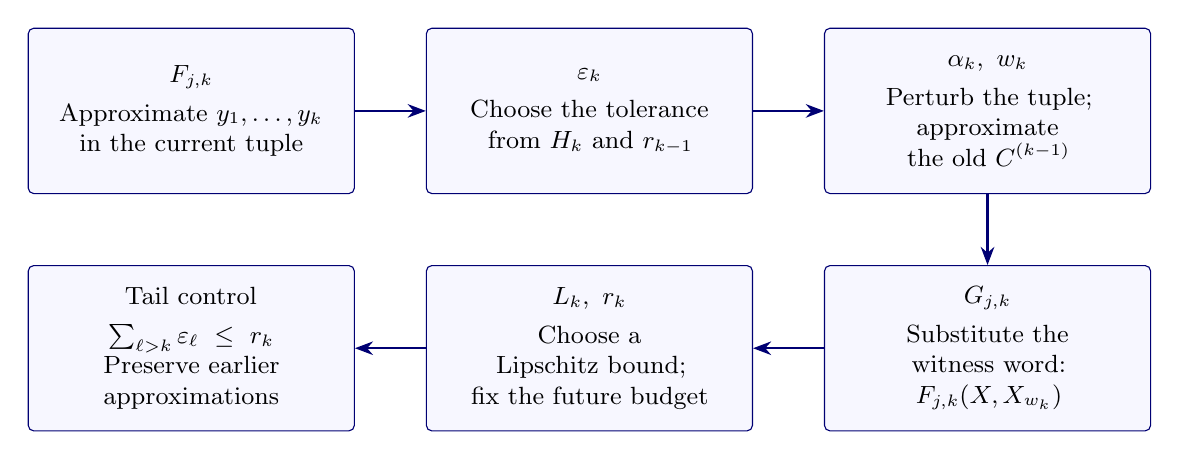
\begin{tikzpicture}[
  stage/.style={draw=blue!45!black, rounded corners=2pt,
    fill=blue!3, text width=3.65cm, minimum height=2.1cm,
    align=center, inner sep=7pt, font=\small},
  choice/.style={-{Stealth[length=2.3mm]}, thick, draw=blue!45!black},
  node distance=9mm and 9mm
]
\node[stage] (old) {$F_{j,k}$\\[3pt]
  Approximate $y_1,\ldots,y_k$\\in the current tuple};
\node[stage, right=of old] (epsilon) {$\varepsilon_k$\\[3pt]
  Choose the tolerance\\from $H_k$ and $r_{k-1}$};
\node[stage, right=of epsilon] (word) {$\alpha_k,\ w_k$\\[3pt]
  Perturb the tuple;\\approximate the old $C^{(k-1)}$};
\node[stage, below=of word] (new) {$G_{j,k}$\\[3pt]
  Substitute the witness word:\\
  $F_{j,k}(X,X_{w_k})$};
\node[stage, below=of epsilon] (budget) {$L_k,\ r_k$\\[3pt]
  Choose a\\Lipschitz bound;\\fix the future budget};
\node[stage, below=of old] (tail) {Tail control\\[3pt]
  $\sum_{\ell>k}\varepsilon_\ell\leq r_k$\\
  Preserve earlier approximations};
\draw[choice] (old) -- (epsilon);
\draw[choice] (epsilon) -- (word);
\draw[choice] (word) -- (new);
\draw[choice] (new) -- (budget);
\draw[choice] (budget) -- (tail);
\end{tikzpicture}

\caption{The choices at stage $k$ follow the arrows.  The witness
word $w_k$ is found only after $\varepsilon_k$ is fixed.  A longer
witness word may increase the Lipschitz bound $L_k$ of the substituted
polynomials $G_{j,k}$, so its length affects the future budget $r_k$
only.  This budget bounds the total change after stage $k$ and
preserves the target approximations in the limit.}
\label{fig:iteration}
\end{figure}

For $\ell>k$, the geometric decrease of the budgets gives
\[
 \varepsilon_\ell<\frac{r_{\ell-1}}2
       \leq \frac{r_k}{2^{\ell-k}}.
\]
Using \eqref{eq:stage-perturbation}, we therefore obtain, for $p>k$,
\[
 \max_j\norm{A_j^{(p)}-A_j^{(k)}}
 \leq\sum_{\ell=k+1}^{p}\varepsilon_\ell
 \leq r_k.
\]
Since $r_k\leq2^{-k}r_0$, each sequence $(A_j^{(k)})_k$ converges in
operator norm to a unitary $A_j^{(\infty)}$, and
\begin{equation}
\label{eq:generator-tail}
 \max_j\norm{A_j^{(\infty)}-A_j^{(k)}}\leq r_k.
\end{equation}
The limits are unitaries because the unitary group is norm closed.
For every nonidentity reduced word $v\in\F_n$,
\[
 \tau(A_v^{(\infty)})
   =\lim_{k\to\infty}\tau(A_v^{(k)})=0,
\]
by operator-norm continuity of each fixed word evaluation and of
the trace.  Thus the limiting tuple has the free Haar word
distribution.

It remains to prove that this tuple generates $M$.  For every
$j\leq k$, equations \eqref{eq:stage-new-approximation},
\eqref{eq:future-budget}, and \eqref{eq:generator-tail} yield
\begin{align}
\label{eq:limit-target-approximation}
 \normtwo{G_{j,k}(A^{(\infty)})-y_j}
 &\leq
 \normtwo{G_{j,k}(A^{(\infty)})-G_{j,k}(A^{(k)})}
  +\normtwo{G_{j,k}(A^{(k)})-y_j}
 \notag\\
 &\leq L_k r_k+2\cdot2^{-k}
 \leq3\cdot2^{-k}.
\end{align}
Fixing $j$ and letting $k\to\infty$ through $k\geq j$ shows that
$y_j$ belongs to the $L^2$ closure of the word algebra of
$A^{(\infty)}$.  Since the $y_j$ are dense, this word algebra is
dense in all of $L^2(M,\tau)$.

To pass from this density to von Neumann generation, set
$N=W^*(A_1^{(\infty)},\ldots,A_n^{(\infty)})$.  The standard
finite-trace conditional expectation $E_N:M\to N$ is
trace-preserving and extends to the orthogonal projection of
$L^2(M,\tau)$ onto $L^2(N,\tau)$.  In particular it is
$L^2$-contractive and fixes every element of $N$.
Each $G_{j,k}(A^{(\infty)})$ belongs to $N$, so
\[
 \normtwo{E_N(y_j)-y_j}
 \leq 2\normtwo{G_{j,k}(A^{(\infty)})-y_j}
 \longrightarrow0.
\]
Hence the projection fixes the dense family $(y_j)$ and is the
identity on $L^2(M,\tau)$.  For $x\in M$, this implies
$E_N(x)=x$ by faithfulness of $\tau$, and therefore $N=M$.

The limiting tuple is now a freely generating Haar $n$-tuple in
$M$.  Lemma~\ref{lem:haar-identification} supplies a unital
trace-preserving normal $*$-isomorphism from $L(\F_n)$ onto
$M=L(\F_{n+1})$, proving the theorem.
\end{proof}

\begin{remark}
Only the first $n$ generators are required to converge in operator
norm.  The completions $C^{(k)}$ may vary without a limit.
The target approximations are in $L^2$, and the conditional
expectation argument permits the operator norms of the
approximating polynomials to grow with $k$.
\end{remark}

\section{Amplification to rank two}\label{sec:amplification}
We recall the amplification convention for a $\mathrm{II}_1$ factor
$(Q,\tau_Q)$. Let $\Tr$ be the usual semifinite trace on $B(\ell^2)$,
normalized to give every rank-one projection trace one. For $t>0$,
choose a projection $p$ in the stabilized factor with
$(\tau_Q\otimes\Tr)(p)=t$ and set
\[
 Q^t=p\bigl(Q\,\overline\otimes\,B(\ell^2)\bigr)p,
 \qquad
 \tau_{Q^t}=t^{-1}(\tau_Q\otimes\Tr)\big|_{Q^t}.
\]
Projections of every positive finite trace exist in this stabilized
factor. Equivalence of projections of equal finite trace makes the
normalized corner independent of the choice of $p$, up to a normal
trace-preserving $*$-isomorphism.

Amplification respects normal tracial isomorphisms. Indeed, if
$\Theta:Q\to R$ is such an isomorphism, the normal tensor-product map
$\Theta\otimes\mathrm{id}$ preserves the semifinite trace and sends
$p$ to a projection $p'$ of the same trace $t$. Its restriction is an
onto normal isomorphism between the corresponding corners. It sends
the corner unit $p$ to $p'$ and preserves their traces normalized by
$t^{-1}$. We denote the resulting map by $\Theta^t:Q^t\to R^t$.

For real $s>1$, let $N_s=L(\F_s)$ be the interpolated free group factor,
with the usual group factor at integer parameters. The established
amplification formula is
\begin{equation}\label{eq:interpolation-formulas}
 N_s^t\cong N_{1+(s-1)t^{-2}}
 \qquad(s>1,\ t>0);
\end{equation}
see \cite[Theorem~2.4]{dykema1994}. This is an unconditional
isomorphism formula for the interpolated family and does not assume
that distinct parameters determine distinct isomorphism classes.
It is the only interpolation theorem used in the proof of
Theorem~\ref{thm:main}.

\begin{proof}[Proof of Theorem~\ref{thm:main}]
Apply Theorem~\ref{thm:rank-step} with $n=3$ and $n=4$ to obtain
\[
 N_3\cong N_4\cong N_5.
\]
Let $\Theta:N_3\to N_5$ be the composition of these normal
trace-preserving isomorphisms. Amplifying by $\sqrt2$ gives a
unital normal trace-preserving isomorphism
\[
 \Theta^{\sqrt2}:N_3^{\sqrt2}\longrightarrow N_5^{\sqrt2}.
\]
Formula~\eqref{eq:interpolation-formulas} identifies its domain and
range as follows:
\[
 N_3^{\sqrt2}\cong N_{1+(3-1)/2}=N_2,
 \qquad
 N_5^{\sqrt2}\cong N_{1+(5-1)/2}=N_3.
\]
These identifications and the amplified map compose to give
$\Phi:L(\F_2)\to L(\F_3)$. Every map in the composition is a unital
normal trace-preserving $*$-isomorphism. Thus $\Phi$ is bijective
and has all the asserted properties.
\end{proof}


For completeness, we record the consequences for the whole interpolated
family. Put $N_\infty=L(\F_\infty)$ and, for a $\mathrm{II}_1$ factor $Q$,
define its fundamental group by
\[
 \mathcal F(Q)=\{t>0:Q^t\cong Q\}.
\]
Here and below the isomorphisms are normal and preserve the normalized
traces. The classical free group factor alternative says that either
all $N_r$, $1<r\leq\infty$, are isomorphic, or $N_r\not\cong N_s$
whenever $1<r<s\leq\infty$. The inclusion of the infinite parameter
uses R\u adulescu's dichotomy \cite[Corollary~4.7]{radulescu1994},
restated explicitly in \cite[Theorem~1.1]{goldbring_pi2025}.
Dykema's corresponding dichotomy \cite[Corollary~4.2]{dykema1994}
is stated for finite parameters.

\begin{corollary}\label{cor:all-interpolated}
For all $1<r,s\leq\infty$ there is a unital normal trace-preserving
$*$-isomorphism $L(\F_r)\cong L(\F_s)$. Moreover,
\[
 \mathcal F\bigl(L(\F_r)\bigr)=\R_{>0}
 \qquad(1<r\leq\infty).
\]
\end{corollary}
\begin{proof}
Theorem~\ref{thm:main} rules out the pairwise-nonisomorphic alternative,
so all parameters, including $\infty$, give the same isomorphism class.
For finite $r>1$ and every $t>0$, formula~\eqref{eq:interpolation-formulas}
then gives
\[
 N_r^t\cong N_{1+(r-1)t^{-2}}\cong N_r.
\]
Thus $\mathcal F(N_r)=\R_{>0}$. Finally, $N_\infty\cong N_2$ and
functoriality of amplification give
$N_\infty^t\cong N_2^t\cong N_2\cong N_\infty$ for every $t>0$.
\end{proof}

\section{Free entropy dimensions and von Neumann generators}
\label{sec:entropy-dimensions}

For a bounded self-adjoint tuple $Z$ in a tracial von Neumann algebra,
let $\delta(Z)$ and $\delta_0(Z)$ denote Voiculescu's microstates free
entropy dimensions. The second is the modified version using entropy
in the presence of the perturbing semicircular family. Write $\delta^*(Z)$
and $\delta^\star(Z)$ for the nonmicrostates dimensions defined through
nonmicrostates free entropy $\chi^*$ and free Fisher information
$\Phi^*$, respectively. We use the conventions in
\cite[Section~2.4]{voiculescu2002entropy} and
\cite[Section~4.1.1]{connes_shlyakhtenko2005}.

By their definitions, all four quantities depend only on the joint
tracial $*$-distribution of the tuple. This is weaker than invariance
under a change of von Neumann generators: two tuples can generate the
same von Neumann algebra without having the same joint distribution.
The isomorphisms proved above show that the four dimensions do change
under such a replacement.

\begin{corollary}[Dependence on von Neumann generators]
\label{cor:entropy-dimensions}
Let $M=L(\F_2)$ with its canonical trace. For every integer $n\geq2$
there are a self-adjoint $n$-tuple $X^{(n)}$ and a self-adjoint
$2n$-tuple $Y^{(n)}$ such that
\[
 W^*(X^{(n)})=W^*(Y^{(n)})=M
\]
and
\[
 \delta(X^{(n)})=\delta_0(X^{(n)})=n,
 \qquad
 \delta^*(Y^{(n)})=\delta^\star(Y^{(n)})=n.
\]
Consequently, none of $\delta,\delta_0,\delta^*,\delta^\star$ is
invariant under changing a finite self-adjoint $W^*$-generating tuple
of a tracial von Neumann algebra. Each takes unbounded values on such
generating tuples of the single factor $L(\F_2)$.
\end{corollary}

\begin{proof}
Fix an integer $n\geq2$. Theorem~\ref{thm:main} and successive
applications of Theorem~\ref{thm:rank-step} provide a unital normal
trace-preserving $*$-isomorphism
\[
 \theta_n:L(\F_n)\longrightarrow M;
\]
for $n=2$ we may take the identity. If $Z$ is any finite self-adjoint tuple in
$L(\F_n)$ and $p$ is a noncommutative $*$-polynomial, then
\[
 \tau_M\bigl(p(\theta_n(Z))\bigr)=\tau_{L(\F_n)}\bigl(p(Z)\bigr).
\]
Thus coordinatewise transport by $\theta_n$ preserves the joint
tracial $*$-distribution and hence each of the four dimensions.
Normality and surjectivity also give
$W^*(\theta_n(Z))=\theta_n(W^*(Z))$.

Let $S^{(n)}=(s_1,\ldots,s_n)$ be a freely independent variance-one semicircular
tuple in the semicircular realization of $L(\F_n)$
\cite[Remarks~1.10--1.11]{voiculescu1990}. It generates $L(\F_n)$ as a von Neumann algebra,
and the standard semicircular computations give
\[
 \delta(S^{(n)})=\delta_0(S^{(n)})=n;
\]
see \cite[Section~2.4(c) and (d)]{voiculescu2002entropy} for $\delta$
and \cite[Section~5, opening paragraph]{brannan_elzinga_harris_yamashita2023}
for $\delta_0$. Set $X^{(n)}=\theta_n(S^{(n)})$. The preceding
transport observations prove the required generation and the two
microstates values.

For the nonmicrostates dimensions, let $u_1,\ldots,u_n$ be the
canonical group unitaries in $L(\F_n)$ and put
\[
 a_j=\frac{u_j+u_j^*}{2},\qquad
 b_j=\frac{u_j-u_j^*}{2\ii},\qquad
 G^{(n)}=(a_1,b_1,\ldots,a_n,b_n).
\]
The entries are self-adjoint, and $u_j=a_j+\ii b_j$ and
$u_j^*=a_j-\ii b_j$. Hence they generate the algebraic group algebra
$\C\F_n$ as a unital $*$-algebra, and generate $L(\F_n)$ as a von
Neumann algebra. Apply Mineyev and Shlyakhtenko's group-algebra theorem
\cite[Theorem~4.1]{mineyev_shlyakhtenko2005} to this tuple, before
transporting it. It gives
\[
 \delta^*(G^{(n)})=\delta^\star(G^{(n)})
 =\beta_1^{(2)}(\F_n)-\beta_0^{(2)}(\F_n)+1=n.
\]
Here $\beta_0^{(2)}(\F_n)=0$ and $\beta_1^{(2)}(\F_n)=n-1$ are the
usual $L^2$-Betti numbers of the free group; see
\cite[Section~2.1.1]{connes_shlyakhtenko2005}. Define
$Y^{(n)}=\theta_n(G^{(n)})$. Again its joint tracial $*$-distribution
is unchanged and it generates $M$, proving the remaining assertions.
Taking $n=2$ and $n=3$ gives different values on generators of the
same factor, and letting $n$ grow gives unboundedness.
\end{proof}

The nonmicrostates computation uses algebraic generators of
$\C\F_n$ before transport. The transported tuples all generate
$L(\F_2)$ as a von Neumann algebra, but their algebraic $*$-algebras
are not held fixed as $n$ varies. Thus the corollary concerns
$W^*$-generation and is compatible with the algebraic-generator
invariance in \cite[Theorem~4.1]{mineyev_shlyakhtenko2005}.


\bibliographystyle{plain}
\bibliography{references}
\end{document}
